\documentclass[tikz,border=3pt]{standalone}
\usepackage[T1]{fontenc}
\usepackage{mathptmx}
\usepackage{tikz,pgfplots}
\usetikzlibrary{arrows.meta,positioning,calc,fit,backgrounds,shapes.geometric}
\pgfplotsset{compat=1.18}
\definecolor{forest}{HTML}{346E57}
\definecolor{sage}{HTML}{E8EFEA}
\definecolor{clay}{HTML}{AC653F}
\definecolor{sand}{HTML}{F4EAE2}
\definecolor{ink}{HTML}{252525}
\definecolor{light}{HTML}{F5F5F3}
\definecolor{gridgray}{HTML}{D8DAD6}
\tikzset{box/.style={draw=ink!70,line width=.5pt,rectangle,rounded corners=1pt,fill=white,align=center,font=\fontsize{11}{12}\selectfont,inner sep=6pt}, flow/.style={-{Latex[length=2.4mm]},line width=.7pt,draw=ink!80}, data/.style={flow,densely dashed,draw=forest}, label/.style={font=\fontsize{10}{11}\selectfont,fill=white,inner sep=2pt,align=center}}
\hyphenpenalty=10000\exhyphenpenalty=10000\begin{document}
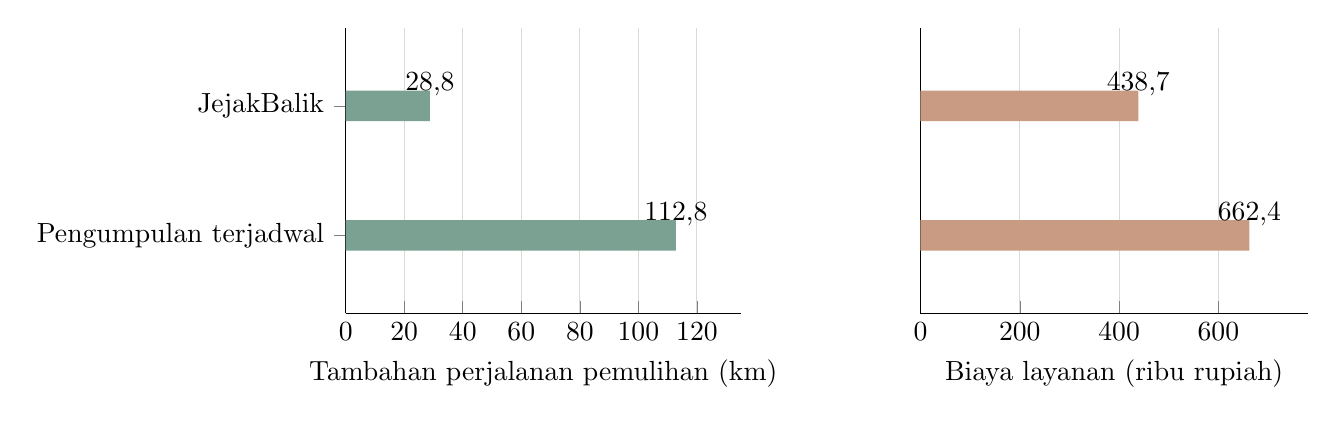
\begin{tikzpicture}
\begin{axis}[width=6.6cm,height=5.2cm,xbar,xmin=0,xmax=135,ytick={1,2},yticklabels={Pengumpulan terjadwal,JejakBalik},ymin=.4,ymax=2.6,bar width=11pt,xlabel={Tambahan perjalanan pemulihan (km)},xlabel style={font=\fontsize{10}{11}\selectfont},tick label style={font=\fontsize{10}{11}\selectfont},axis lines*=left,xmajorgrids=true,grid style={gridgray},nodes near coords,nodes near coords style={font=\fontsize{10}{11}\selectfont,text=black},point meta=explicit symbolic]
\addplot[fill=forest!65,draw=none]coordinates{(112.8,1)[112,8] (28.8,2)[28,8]};
\end{axis}
\begin{axis}[at={(7.3cm,0)},anchor=south west,width=6.5cm,height=5.2cm,xbar,xmin=0,xmax=780,ytick=\empty,ymin=.4,ymax=2.6,bar width=11pt,xlabel={Biaya layanan (ribu rupiah)},xlabel style={font=\fontsize{10}{11}\selectfont},tick label style={font=\fontsize{10}{11}\selectfont},axis lines*=left,xmajorgrids=true,grid style={gridgray},nodes near coords,nodes near coords style={font=\fontsize{10}{11}\selectfont,text=black},point meta=explicit symbolic]
\addplot[fill=clay!65,draw=none]coordinates{(662.4,1)[662,4] (438.7,2)[438,7]};
\end{axis}
\end{tikzpicture}
\end{document}
